\documentclass[12pt, psamsfonts]{amsart}

%-------Packages---------
\usepackage{amssymb,amsfonts}
\usepackage{listings}
\usepackage{fullpage}
\usepackage{tikz-cd}
\usepackage{todonotes}
\usepackage{physics}
\usepackage[all,arc]{xy}
\usepackage{enumerate}
\usepackage{enumitem}
\usepackage{mathrsfs}
\usepackage{theoremref}
\usepackage{graphicx}
\usepackage[bookmarks]{hyperref}

%--------Theorem Environments--------
%theoremstyle{plain} --- default
\newtheorem{thm}{Theorem}[section]
\newtheorem{cor}[thm]{Corollary}
\newtheorem{prop}[thm]{Proposition}
\newtheorem{lem}[thm]{Lemma}
\newtheorem{conj}[thm]{Conjecture}
\newtheorem{quest}[thm]{Question}

\theoremstyle{definition}
\newtheorem{defn}[thm]{Definition}
\newtheorem{defns}[thm]{Definitions}
\newtheorem{con}[thm]{Construction}
\newtheorem{exmp}[thm]{Example}
\newtheorem{exmps}[thm]{Examples}
\newtheorem{notn}[thm]{Notation}
\newtheorem{notns}[thm]{Notations}
\newtheorem{addm}[thm]{Addendum}
\newtheorem*{exer}{Exercise}

\theoremstyle{remark}
\newtheorem{rem}[thm]{Remark}
\newtheorem{rems}[thm]{Remarks}
\newtheorem{warn}[thm]{Warning}
\newtheorem{sch}[thm]{Scholium}

\DeclareMathOperator{\Hom}{Hom}
\DeclareMathOperator{\Id}{Id}
\DeclareMathOperator{\End}{End}
\DeclareMathOperator{\ord}{ord}
\DeclareMathOperator{\Aut}{Aut}

\makeatletter
\let\c@equation\c@thm
\makeatother
\numberwithin{equation}{section}

\bibliographystyle{plain}

\begin{document}

\title{Math 601 (Due 11/13)}
\author{Hidenori Shinohara}
\maketitle

\tableofcontents

\section{Factoring Polynomials with Coefficients in Finite Fields}

\begin{exer}{(Problem 14)}
  For $a \in \mathbb{F}_q$, what are the possible values for $a^{(q - 1)/2}$?
  How many different $a$ take each value?
\end{exer}

\begin{proof}
  Let $\ev{\alpha} = (\mathbb{F}_q)^*$.
  Let $k \in \mathbb{Z}$.
  If $k$ is even, then $(\alpha^{k})^{(q - 1)/2} = (\alpha^{k/2})^{q - 1} = 1$.
  If $k = 2l + 1$ for some $l$, then $(\alpha^{k})^{(q - 1)/2} = \alpha^{l(q - 1)}\cdot\alpha^{(q - 1)/2} = \alpha^{(q - 1) / 2} = -1$ because -1 has degree 2 and $\alpha^{(q - 1)/2}$ is the only element in $\ev{\alpha}$ of degree 2.
  Therefore, 
  \begin{align*}
    a^{(q - 1) / 2} &= \begin{cases}
      0 & (a = 0) \\
      1 & (\exists l \in \mathbb{Z}, a = \alpha^{2l}) \\
      -1 & (\exists l \in \mathbb{Z}, a = \alpha^{2l + 1}).
    \end{cases}
  \end{align*}
  This is well defined because every nonzero element in $\mathbb{Z}_q$ is in $\ev{\alpha}$ and $2 \mid \abs{\ev{\alpha}} = q - 1$, so the parity of the exponent does not depend on the choice of $k$.
  Hence, 1 value gives 0, $(q - 1)/2$ values give 1, and $(q - 1) / 2$ values give $-1$.
\end{proof}

\begin{exer}{(Problem 15)}
  Let $f(x)$ be as in problem 13 and let $h \in \mathbb{F}_q[x]$ be a randomly chosen polynomial.
  What is the probability that $h^{(q^r - 1)/2} = \pm 1$ in the ring $\mathbb{F}_q[x]/(f(x))$.
\end{exer}

\begin{proof}
  As shown in Problem 13 last week, there exists an isomorphism $\Phi: \mathbb{F}_q[x]/(f(x)) \rightarrow \mathbb{F}_q[x]/(f_1(x)) \times \cdots \times \mathbb{F}_q[x]/(f_m(x))$ by the Chinese Remainder Theorem.
  For any $h \in \mathbb{F}_q[x]$, $\Phi(h + (f)) = (h + (f_1), \cdots, h + (f_m))$.
  Moreover, $\Phi(h^{(q - 1)/2} + (f)) = (h^{(q - 1)/2} + (f_1), \cdots, h^{(q - 1)/2} + (f_m))$.
  Therefore, $h^{(q - 1)/2} + (f) = 1$ if and only if $h^{(q - 1)/2} + (f_1), \cdots, h^{(q - 1)/2} + (f_m)$ all equal 1.

  Let $\alpha_1, \cdots, \alpha_m$ be generators of $(\mathbb{F}_q[x]/(f_1(x)))^*, \cdots, (\mathbb{F}_q[x]/(f_m(x)))^*$.
  For each $i$, $h^{(q - 1)/2} + (f_i) = 1$ if and only if $h \in \ev{ \alpha_i^2 }$ by Problem 14.
  Therefore, $h^{(q - 1)/2} + (f) = 1$ if and only if $(h + (f_1), \cdots, h + (f_m)) \in \ev{ \alpha_1^2 } \times \cdots \times \ev{ \alpha_m^2 }$.
  There are exactly $((q^r - 1)/2)^m$ elements that satisfy that.
  Therefore,
  \begin{align*}
    \frac{(\frac{q^r - 1}{2})^m}{(q^r)^m} = \Big(\frac{q^r - 1}{2q^r}\Big)^m = \Big(\frac{1}{2} - \frac{1}{2q^r}\Big)^m.
  \end{align*}
  is the probability that $h^{(q^r - 1)/2} = 1$ in $\mathbb{F}_q[x]/(f(x))$.

  Using the exact same argument, we can derive that the probability that $h^{(q^r - 1)/2} = -1$ is exactly the same value.
\end{proof}

\begin{exer}{(Problem 16)}
  With $f(x)$ as in problem 13, write $f(x) = g_1(x) \cdots g_m(x)$ for the factorization into irreducible factors.
  Express $\gcd(f(x), h^{(q^r - 1)/2} - 1)$ in terms of the $g_i(x)$'s.
\end{exer}

\begin{proof}
  $\gcd(f(x), h^{(q^r - 1)/2} - 1)$ is the product of $g_i(x)$'s that divide $h^{(q^r - 1)/2} - 1$.
  It is divisible by $g_i(x)$ if and only if $h \in \ev{ \alpha_i^2 }$ from Problem 15.
\end{proof}

\begin{exer}{(Problem 17)}
  Describe a probabilistic factoring algorithm which has a very high probability of finding the irreducible factors of a polynomial $f(x) \in \mathbb{F}_q[x]$, provided one knows ahead of time that $f(x)$ is a product of m distinct irreducible polynomials of degree $r$.
\end{exer}

\begin{proof}
  Let $i_0$ be fixed.
  Given a random $h(x) \in \mathbb{F}_q[x]$, the probability that $h^{(q - 1)/2} - 1 \in (f_{i_0})$ is $1/2 - 1/(2q^r)$, which is slightly smaller than 50\%.
  Therefore, it is likely that given a random $h(x) \in \mathbb{F}_q[x]$, the probability that $h^{(q - 1)/2} - 1 \in (f_i)$ for \textit{some} $i$'s is high.
  However, the probability that $h^{(q - 1)/2} - 1 \in (f_i)$ in \textit{all} $i$'s is low.

  In other words, the probability that $h^{(q - 1)/2} - 1$ is a proper divisor of $f$ is high.
  Therefore, we can expect to factor $f(x)$ by 

  \begin{itemize}
    \item
      Step 1: Generate a random polynomial $h(x) \in \mathbb{F}_q[x]/(f(x))$.
    \item
      Step 2: Calculate $h^{(q^r - 1)/2} - 1$.
      This step can be done efficiently by exponentiation by squaring.
    \item
      Step 3: Calculate $d(x) = \gcd(f(x), h^{(q^r - 1)/2} - 1)$.
      This step can be done efficiently by the Euclid algorithm.
    \item
      Step 4: If $1 \leq \deg(d(x)) < \deg(f(x))$, then factorize $f(x)/d(x)$ and $d(x)$ further by going back to Step 1 unless it is degree $r$.
      Otherwise, we were unlucky, so we go back to Step 1.
  \end{itemize}
\end{proof}

\begin{exer}{(Problem 18, 19, 20)}
  \begin{itemize}
    \item
      Problem 18: $(x^{2} + x - 1)^4$
    \item
      Problem 19: $(x^{3} - 25 x^{2} - 35 x + 3)(x^{4} + 4 x^{2} + 5 x + 3)(x^{5} + 4 x^{2} + 8 x + 3)$.
    \item
      Problem 20: $(x^{4} + 4 x^{2} + 5 x + 3)(x^{4} + 15 x^{3} - 16 x^{2} - 27 x - 26)(x^{4} - 3 x^{3} + 9 x^{2} - 23 x + 1)$.
  \end{itemize}
  I used the following Python code to factorize.
  The idea is to use the methods developed in Problem 11 and Problem 17.
  Later, I noticed that I should have added code to check if $f(x)$ is square free, but for some reason, the code was still able to factorize the polynomial for Problem 18.
  \begin{lstlisting}[language=python]
    from sympy import *
    from random import *

    x = symbols('x')

    # Find a random polynomial of degree <= deg in Z_{mod}.
    def randpoly(deg, mod):
        p = poly(0, x, modulus = mod)
        for d in range(deg):
            p = x * p + randint(0, mod - 1)
        return poly(p, x, modulus = mod)

    # Find f^exp % modf in Z_{mod}.
    def polypow(f, exp, modf, mod):
        res = poly(1, x, modulus = mod)
        while exp > 0:
            if exp % 2 == 1:
                quotient, res = div(res * f, modf, modulus = mod)
            quotient, f = div(f * f, modf, modulus = mod)
            exp = exp // 2
        return res

    # Calculate x^(p^n) - x % modf.
    def xqd(p, n, modf):
        res = polypow(x, p**n, modf, p)
        res -= poly(x, x, modulus = p)
        return res


    def factor(f, p, originaldegree, factors):
        # Problem 11
        for n in range(2, originaldegree):
            g = xqd(p, n, f)
            d = gcd(f, g)
            if 1 <= d.degree() < f.degree():
                # We found a proper factor.
                # Factorize further.
                factor(d, p, originaldegree, factors)
                quotient, remainder = div(f, d, modulus = p)
                factor(quotient, p, originaldegree, factors)
                return

        # Problem 17
        for r in range(2, f.degree()):
            if f.degree() % r != 0: continue
            for i in range(10):
                h = randpoly(r, p)
                # Raise h to the power of (p^r - 1)/2.
                h = polypow(h, (p**r - 1) // 2, f, p)
                h = h - poly(1, x, modulus = p)
                d = gcd(f, h)
                if d.degree() == 0 or d.degree() == f.degree():
                    continue
                else:
                    # We found a proper factor.
                    # Factorize further.
                    factor(d, p, originaldegree, factors)
                    quotient, remainder = div(f, d)
                    factor(quotient, p, originaldegree, factors)
                    return
        factors.append(f)

    def factorizepoly(f, mod):
        print("Factorize %s" % f)
        factors = []
        factor(f, mod, f.degree(), factors)
        prod = poly(1, x, modulus = mod)
        for fac in factors:
            prod *= fac
            print(latex(fac))
        if prod != f:
            print("******ERROR!******")
        print()
        return

    f = poly(x**8 + x**7 - x**6 + x**5 + x**4 - x**3 - x**2 - x + 1, x, modulus = 3)
    factorizepoly(f, 3)

    f = poly((x**12+48*x**11+42*x**10+58*x**9+11*x**8+25*x**7+22*x**6+30*x**5+34*x**4+16*x**3+62*x**2+21*x+27), x, modulus = 73)
    factorizepoly(f, 73)

    f = poly((x**12+12*x**11 +25*x**10 + 40*x**9 + 6*x**8 + 15*x**7 + 24*x**6+ 42*x**5 + 8*x**4 + 48*x**3 +68*x**2 + 50*x +68), x, modulus = 73)
    factorizepoly(f, 73)
  \end{lstlisting}
\end{exer}

\section{Galois Theory III}

\begin{exer}{(Problem 1)}
  Prove Proposition 23 part (ii).
\end{exer}

\begin{proof}
  Clearly, $F \subset gK \subset L$ because $g \in \Aut(L / F)$.
  $gK$ is a subfield because $g$ preserves addition, multiplication and multiplicative inverse, so $gK$ is closed under addition, multiplication and multiplicative inverse.

  Let $\phi \in \Aut(L/gK)$.
  Then clearly, $g^{-1}\phi g \in \Aut(L)$.
  $g^{-1}\phi g$ fixes $K$ because $\forall x \in K, (g^{-1}\phi g)(x) = g^{-1}(g(x)) = x$.
  Therefore, $\phi \in g\Aut(L/K)g^{-1}$.

  Let $g\psi g^{-1} \in g\Aut(L/K)g^{-1}$.
  Then $g\psi g^{-1} \in \Aut(L)$.
  For all $g(k) \in g(K)$, $(g\psi g^{-1})(g(k)) = g(\psi(k)) = g(k)$.
  Therefore, $g\psi g^{-1} \in \Aut(L/gK)$.
\end{proof}

\begin{exer}{(Problem 2)}
  Show that the Galois correspondence is order reversing.
\end{exer}

\begin{proof}
  Let $H_1 \subset H_2$ be given.
  Let $x \in K^{H_2}$.
  Then $x$ is fixed by every element in $H_2$.
  Then $x$ is clearly fixed by every element in $H_1$.
  Thus $x \in K^{H_1}$.

  Let $K_1 \subset K_2$.
  Let $\sigma \in \Aut(L/K_2)$.
  Then $\sigma$ clearly fixes $K_1$.
  Thus $\sigma \in \Aut(L/K_1)$.
\end{proof}


\begin{exer}{(Problem 3)}
  Draw a picture showing all the subgroups of the dihedral group with eight elements, $D4 := \ev{a , f: a^4 = 1 = f^2, faf = a^{-1}} \simeq \ev{(1234),(12)(34)} \subset S_4$ showing which are contained in which.
  Now draw a diagram of the corresponding intermediate fields in a Galois extension, $F \subset L$, with Galois group isomorphic to $D_4$ indicating which are ¢ontained in which.
\end{exer}

\begin{proof}
  Figure \ref{fig:problem3}.
  \begin{figure}
    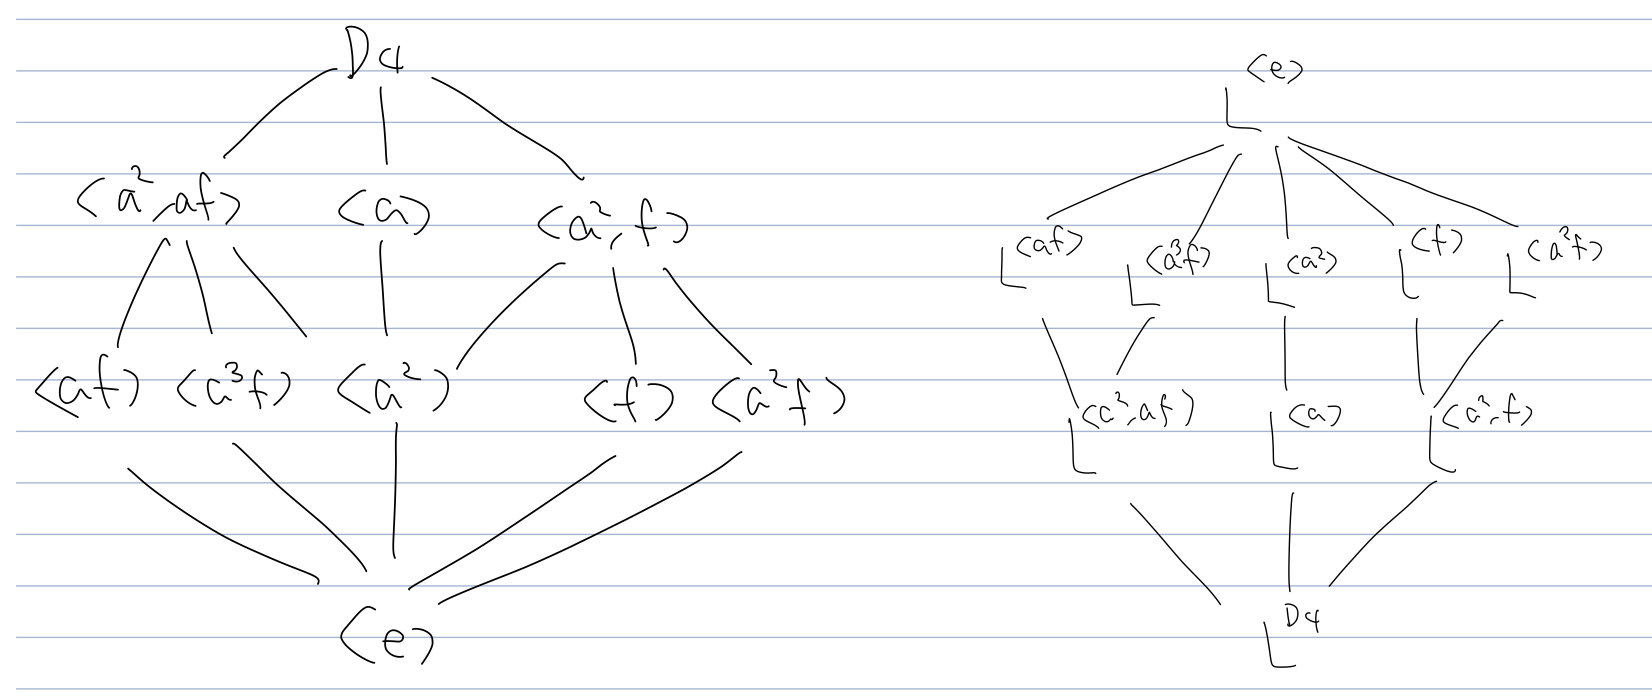
\includegraphics[width=\linewidth]{problem3.jpg}
    \caption{Problem 3}
    \label{fig:problem3}
  \end{figure}
\end{proof}

\begin{exer}{(Problem 4)}
  Let $F \subset M$ be a Galois extension with Galois group isomorphic to the dihedral group with eight elements (denoted D 4 in class).
  Show that there is a tower of intermediate fields, $F \subset K \subset L$ such that $F \subset K$ is Galois and $K \subset L$ is Galois, but $F \subset L$ is not Galois.
\end{exer}

\begin{proof}
  $G_1 = \ev{af}$ is a normal subgroup of $G_2 = \{ e, af, a^2, a^3f \}$ because the index is 2.
  Similarly, $G_2$ is a normal subgroup of $D_4$ because the index is 2.
  However, $G_1$ is not a normal subgroup of $D_4$.
  (For instance, $f\ev{af}f^{-1} = \ev{fa}$ ,but $af \ne fa$.)
  By the Fundamental Theorem of Galois Theory, $L^{G_1}$ and $L^{G_2}$ are intermediate fields.
  By Proposition 23(iii), $L^{G_2} \subset L^{G_1}$ and $L^{D_4} \subset L^{G_2}$ is Galois, but $L^{D_4} \subset L^{G_1}$ is not Galois.
\end{proof}

\begin{exer}{(Problem 5)}
  Let $F \subset M$ be a Galois extension with Galois group isomorphic to the symmetric group $S_4$.
  Let $H = \ev{(123)} \subset S_4$.
  Make a list of the intermediate fields in the extension, $F \subset M^H$.
  For each intermediate field $L$ indicate whether or not $F \subset L$ is Galois and whether or not $L \subset M^H$ is Galois.
\end{exer}

\begin{proof}
  There are only 4 subgroups of $S_4$ that contain $S_3$.
  They are $H, S_3, A_4, S_4$.

  Clearly, $M^H \subset M^H$ is Galois.
  $H$ is not a normal subgroup of $S_4$ because $(14)(12)(14) \notin H$.
  Therefore, $F \subset M^H$ is not Galois.

  $S_3 = \{ e, (12), (13), (23), (123), (132) \}$ is a proper subgroup of $S_4$ that contains $H$ properly.
  Therefore, $F \subsetneq M^{S_3} \subsetneq M^H$.
  Since $[S_3:H] = 2$, $H$ is a normal subgroup of $S_3$.
  Therefore, $M^{S_3} \subset M^{H}$ is Galois.
  $S_3$ is not a normal subgroup of $S_4$ because $(14)(12)(14) \notin S_3$.
  Therefore, $F \subset M^{S_3}$ is not Galois.

  $A_4$ is a normal subgroup of $H$ because the index is 2.
  Therefore, $F \subset M^{A_4}$ is Galois.
  $H$ is not a normal subgroup of $A_4$ because $((12)(34))(23)((12)(34)) = (14) \notin H$.
  Therefore, $M^{A_4} \subset M_h$ is not Galois.
\end{proof}


\end{document}
